\documentclass[dcc]{fcfmcourse}
\usepackage{teoria}
\usepackage[utf8x]{inputenc}
\usepackage{amsmath}
\usepackage{amsfonts,setspace}
\usepackage{listings}
\usepackage{color}
\usepackage{cancel}
\usepackage{epstopdf}
\usepackage{qtree}
\usepackage{fancyhdr}
\usepackage{tikz}
\usepackage{hyperref}
\usetikzlibrary{automata,positioning}
\pagestyle{fancy}
\cfoot{``The more I study, the more insatiable do I feel my genius for it to be." \\Ada Lovelace}
\definecolor{pblue}{rgb}{0.13,0.13,1}
\definecolor{pgreen}{rgb}{0,0.5,0}
\definecolor{porange}{rgb}{0.9,0.5,0}
\definecolor{pgrey}{rgb}{0.46,0.45,0.48}

\lstset{language=Java,
  showspaces=false,
  showtabs=false,
  breaklines=true,
  showstringspaces=false,
  breakatwhitespace=true,
  commentstyle=\color{porange},
  keywordstyle=\color{pblue},
  stringstyle=\color{pgreen},
  basicstyle=\ttfamily,
  moredelim=[il][\textcolor{pgrey}]{$ $},
  moredelim=[is][\textcolor{pgrey}]{\%\%}{\%\%}
}

\newenvironment{codebox} {\small \ttfamily \obeylines \begingroup \setstretch{-2.4}} {\endgroup}

\title{Auxiliar Extra}
\course[CC3102]{Teoría de la Computación}
\professor{Gonzalo Navarro}
\assistant{Manuel Cáceres}
\assistant{Ian Letter}

% Si pasas el comando usedate a la clase, la fecha aparecerá bajo la lista de auxiliares.
% Puedes usar el formato de fecha por defecto de latex (y traducirla usando babel)
% o puedes escribir lo que quieras con el comando \date.
% \date{1 de Septiembre, 2015}

\begin{document}
\maketitle
\begin{center}
27 de Octubre del 2016
\end{center}
\vspace{-1ex}
\begin{problems}
\problem Considere la siguiente gramática no ambigüa de paréntesis bien balanceados
\begin{center}
$S \rightarrow \epsilon | (S)S$
\end{center}
\begin{enumerate}[a)]
    \item Construya el autómata equivalente con la conversión $GLC \rightarrow_{LL(0)} AP$
    \item Construya el autómata equivalente con la conversión $GLC \rightarrow_{LR(0)} AP$
    \item ¿Son deterministas los autómatas obtenidos? ¿Qué puede decir respecto a las conversiones $LL(0)$ y $LR(0)$ de gramáticas no ambiguas? ¿Y si la gramática es ambigüa?
\end{enumerate}
\problem Considere el siguiente lenguaje:
\begin{center}
$\mathcal{L} = \{w \in \{a,b\}^* \colon \#_{a}(w) \not= \#_{b}(w)\}$
\end{center}
\begin{enumerate}[a)]
    \item Construya una GLC que genere $\mathcal{L}$
    \item Construya un AP que acepte $\mathcal{L}$
\end{enumerate}
\problem Considere el siguiente lenguaje:
\begin{center}
$\mathcal{L} = \{a^ib^jc^k \colon i=j\lor j=k\}$
\end{center}
\begin{enumerate}[a)]
    \item Demuestre que $\mathcal{L}$ es libre del contexto
    \item Construya una GLC que genere $\mathcal{L}$
    \item Construya un AP que acepte $\mathcal{L}$
\end{enumerate}
\problem Demuestre que los siguientes lenguajes no son libres del contexto:
\begin{enumerate}[a)]
    \item $\{w \in \{a,b,c\}^* \colon \#_{a}(w) \le \#_{b}(w) \le \#_{c}(w)\}$
    \item $\{a^{f} \colon f \text{ es un número de fibonacci}\}$
    \item $\{w \in \{a,b,c\}^* \colon \#_{a}(w) = \#_{b}(w) = \#_{c}(w)\}$
\end{enumerate}
\end{problems}
\newpage
\begin{center}
{\huge \underline{Soluciones}}
\begin{problems}
\problem 
\begin{enumerate}[a)]
    \item Este autómata : \\
    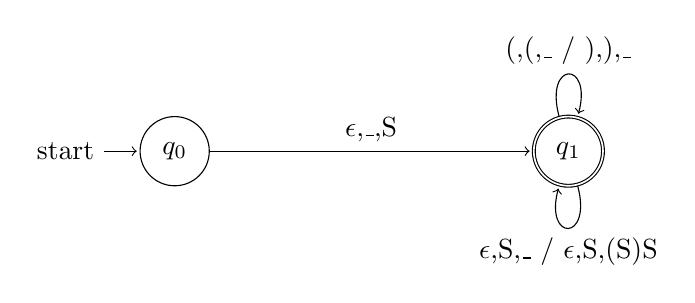
\begin{tikzpicture}[shorten >=1pt,node distance=5cm,on grid,auto] 
   \node[state,initial] (q_0)	{$q_0$}; 
   \node[state,accepting] (q_1) [right of=q_0]  {$q_1$}; 
    \path[->] 
    %(q_0) edge [loop above] node  {a,\_,a\ /\ b,\_,b\ /\ c,\_,c} (q_0)
    (q_0) edge node  {$\epsilon$,\_,S} (q_1)
    (q_1) edge [loop above] node  {(,(,\_\ /\ ),),\_} (q_1)
    (q_1) edge [loop below] node  {$\epsilon$,S,\_\ /\ $\epsilon$,S,(S)S} (q_1);
    \end{tikzpicture}
    \item Este autómata : \\
    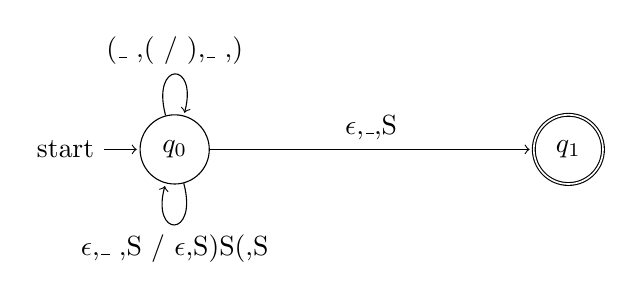
\begin{tikzpicture}[shorten >=1pt,node distance=5cm,on grid,auto] 
   \node[state,initial] (q_0)	{$q_0$}; 
   \node[state,accepting] (q_1) [right of=q_0]  {$q_1$}; 
    \path[->] 
    %(q_0) edge [loop above] node  {a,\_,a\ /\ b,\_,b\ /\ c,\_,c} (q_0)
    (q_0) edge node  {$\epsilon$,\_,S} (q_1)
    (q_0) edge [loop above] node  {(\_ ,(\ /\ ),\_ ,)} (q_0)
    (q_0) edge [loop below] node  {$\epsilon$,\_ ,S\ /\ $\epsilon$,S)S(,S} (q_0);
    \end{tikzpicture}
    \item 
    \begin{itemize}
        \item En el primer autómata colisionan las dos transiciones de aplicación de reglas (del estado $q_{1}$).\\
        En el segundo autómata la primera transición de desaplicación de reglas colisiona con todas las demás.\\
        Por lo tanto, ambos son no deterministas.
        \item Las transformaciones $LL(0)$ y $LR(0)$ a partir de gramáticas no ambiguas no necesariamente generan APs deterministas, de hecho podemos decir que para:
        \begin{itemize}
            \item $LL(0)$, si un no terminal tiene más de una derivación el AP es no determinista.
            \item $LR(0)$, si existe algún no terminal que derive a $\epsilon$, el AP es no determinista.
        \end{itemize}
        \item Si la gramática es ambigua, significa que existe un $w$ derivado de la gramática que tiene dos árboles de derivación diferentes, y por lo tanto un no terminal posee más de una regla de reescritura, es decir, la conversión $LL(0)$ es no determinista.
    \end{itemize}
\end{enumerate}
\newpage
\problem
\begin{enumerate}[a)]
    \item Esta gramática:
    \begin{align*}
        S &\rightarrow A|B& \text{deriva más a's que b's o mas b's que a's}\\
        A &\rightarrow aE|aA|bAA&\\
        B &\rightarrow bE|bA|aBB&\\
        E &\rightarrow aEbE|bEaE|\epsilon& \text{igual número de a's y b's\footnotemark }
    \end{align*}
    \footnotetext{gracias a Daniel por dar estas reglas.}
    \item Este autómata:
    \begin{center}
\begin{tikzpicture}[scale=0.2]
\tikzstyle{every node}+=[inner sep=0pt]
\draw [black] (12,-23.4) circle (3);
\draw [black] (39.8,-5) circle (3);
\draw [black] (39.8,-24.3) circle (3);
\draw [black] (39.8,-42.8) circle (3);
\draw [black] (66.1,-22.6) circle (3);
\draw [black] (66.1,-22.6) circle (2.4);
\draw [black] (14.5,-21.74) -- (37.3,-6.66);
\fill [black] (37.3,-6.66) -- (36.36,-6.68) -- (36.91,-7.51);
\draw (28.35,-14.7) node [below] {$a,\_,\$$};
\draw [black] (14.46,-25.12) -- (37.34,-41.08);
\fill [black] (37.34,-41.08) -- (36.97,-40.22) -- (36.4,-41.04);
\draw (23.4,-33.6) node [below] {$b,\_,\$$};
\draw [black] (39.8,-8) -- (39.8,-21.3);
\fill [black] (39.8,-21.3) -- (40.3,-20.5) -- (39.3,-20.5);
\draw (39.3,-14.65) node [left] {$b,\$,\$$};
\draw [black] (39.8,-39.8) -- (39.8,-27.3);
\fill [black] (39.8,-27.3) -- (39.3,-28.1) -- (40.3,-28.1);
\draw (40.3,-33.55) node [right] {$a,\$,\$$};
\draw [black] (42.29,-6.67) -- (63.61,-20.93);
\fill [black] (63.61,-20.93) -- (63.22,-20.07) -- (62.66,-20.9);
\draw (50.05,-14.3) node [below] {$\epsilon,\_,\_$};
\draw [black] (42.18,-40.97) -- (63.72,-24.43);
\fill [black] (63.72,-24.43) -- (62.78,-24.52) -- (63.39,-25.31);
\draw (55.85,-33.2) node [below] {$\epsilon,\_,\_$};
\draw [black] (67.717,-20.087) arc (174.96376:-113.03624:2.25);
\draw (72.53,-17.86) node [right] {$\epsilon,\$|X,\_$};
\fill [black] (69.08,-22.36) -- (69.83,-22.92) -- (69.92,-21.93);
\draw [black] (41.892,-2.866) arc (163.29005:-124.70995:2.25);
\draw (46.93,-2.02) node [right] {$a,\_,X$};
\fill [black] (42.77,-5.36) -- (43.39,-6.07) -- (43.68,-5.11);
\draw [black] (36.905,-5.742) arc (312.11134:24.11134:2.25);
\draw (32.45,-3.27) node [left] {$b,X,\_$};
\fill [black] (37.45,-3.15) -- (37.28,-2.23) -- (36.54,-2.9);
\draw [black] (42.698,-43.528) arc (103.63546:-184.36454:2.25);
\draw (45.49,-48.61) node [right] {$b,\_,X$};
\fill [black] (40.99,-45.54) -- (40.69,-46.44) -- (41.66,-46.2);
\draw [black] (37.767,-44.99) arc (-15.14554:-303.14554:2.25);
\draw (32.74,-46.04) node [left] {$a,X,\_$};
\fill [black] (36.83,-42.52) -- (36.18,-41.83) -- (35.92,-42.79);
\draw [black] (39.8,-21.3) -- (39.8,-8);
\fill [black] (39.8,-8) -- (39.3,-8.8) -- (40.3,-8.8);
\draw (40.3,-14.65) node [right] {$a,\$,\$$};
\draw [black] (39.8,-27.3) -- (39.8,-39.8);
\fill [black] (39.8,-39.8) -- (40.3,-39) -- (39.3,-39);
\draw (39.3,-33.55) node [left] {$b,\$,\$$};
\end{tikzpicture}
\end{center}
\footnote{gracias a Cristobal por resumir un par de transiciones.}La idea del autómata es que el estado de arriba mantiene el invariante de haber visto más a's que b's el de al medio la misma cantidad y el de abajo más b's que a's.\\
Es interesante notar dos técnicas de construcción de autómatas presentes aquí:
\begin{itemize}
    \item El uso de un símbolo inicial($\$$) que indica el tope de la pila.
    \item Un estado final que desapila lo que tiene.
\end{itemize}
\end{enumerate}
\newpage
\problem
\begin{enumerate}[a)]
    \item Sabemos que $a^nb^n$ es libre del contexto. Como la concatenación de $LLC$ es $LLC$ entonces $a^nb^nc^*$ es libre del contexto. De manera análoga mostramos que $a^*b^nc^n$. Finalmente como la unión de $LLC$ es $LLC$, $\mathcal{L}$ es $LLC$.
    \item Esta gramática:
    \begin{align*}
        S &\rightarrow BC|AD&\\
        B &\rightarrow aBb|\epsilon& \text{deriva $a^nb^n$}\\
        D &\rightarrow bDc|\epsilon& \text{deriva $b^nc^n$}\\
        C &\rightarrow Cc|\epsilon& \text{deriva $c^*$}\\
        A &\rightarrow Aa|\epsilon& \text{deriva $a^*$}
    \end{align*}
    \item Este autómata:
    \begin{center}
\begin{tikzpicture}[scale=0.2]
\tikzstyle{every node}+=[inner sep=0pt]
\draw [black] (7.3,-26) circle (3);
\draw [black] (20.4,-12) circle (3);
\draw [black] (42.8,-11.8) circle (3);
\draw [black] (62.4,-11.8) circle (3);
\draw [black] (62.4,-11.8) circle (2.4);
\draw [black] (20.2,-35.8) circle (3);
\draw [black] (42.8,-35.8) circle (3);
\draw [black] (63.4,-35.8) circle (3);
\draw [black] (63.4,-35.8) circle (2.4);
\draw [black] (9.35,-23.81) -- (18.35,-14.19);
\fill [black] (18.35,-14.19) -- (17.44,-14.43) -- (18.17,-15.12);
\draw (14.38,-20.47) node [right] {$\epsilon,\_,\_$};
\draw [black] (9.69,-27.81) -- (17.81,-33.99);
\fill [black] (17.81,-33.99) -- (17.48,-33.1) -- (16.87,-33.9);
\draw (10.85,-31.4) node [below] {$\epsilon,\_,\_$};
\draw [black] (18.509,-9.686) arc (246.99462:-41.00538:2.25);
\draw (16.79,-4.68) node [above] {$a,\_,X$};
\fill [black] (21.09,-9.09) -- (21.86,-8.55) -- (20.94,-8.16);
\draw [black] (21.064,-38.661) arc (44.53768:-243.46232:2.25);
\draw (17.8,-43.23) node [below] {$a,\_,\_$};
\fill [black] (18.45,-38.23) -- (17.53,-38.43) -- (18.24,-39.14);
\draw [black] (23.4,-11.97) -- (39.8,-11.83);
\fill [black] (39.8,-11.83) -- (39,-11.33) -- (39,-12.33);
\draw (31.6,-12.43) node [below] {$\epsilon,\_,\_$};
\draw [black] (42.09,-8.897) arc (221.47119:-66.52881:2.25);
\draw (46.3,-4.45) node [above] {$b,X,\_$};
\fill [black] (44.67,-9.47) -- (45.6,-9.32) -- (44.94,-8.57);
\draw [black] (45.8,-11.8) -- (59.4,-11.8);
\fill [black] (59.4,-11.8) -- (58.6,-11.3) -- (58.6,-12.3);
\draw (52.6,-12.3) node [below] {$\epsilon,\_,\_$};
\draw [black] (23.2,-35.8) -- (39.8,-35.8);
\fill [black] (39.8,-35.8) -- (39,-35.3) -- (39,-36.3);
\draw (31.5,-36.3) node [below] {$\epsilon,\_,\_$};
\draw [black] (44.396,-38.327) arc (60.00901:-227.99099:2.25);
\draw (44.17,-43.28) node [below] {$b,\_,X$};
\fill [black] (41.77,-38.6) -- (40.93,-39.05) -- (41.8,-39.55);
\draw [black] (45.8,-35.8) -- (60.4,-35.8);
\fill [black] (60.4,-35.8) -- (59.6,-35.3) -- (59.6,-36.3);
\draw (53.1,-36.3) node [below] {$\epsilon,\_,\_$};
\draw [black] (64.142,-38.695) arc (42.11134:-245.88866:2.25);
\draw (60.13,-43.17) node [below] {$c,X,\_$};
\fill [black] (61.55,-38.15) -- (60.63,-38.32) -- (61.3,-39.06);
\draw [black] (62.24,-8.816) arc (210.80141:-77.19859:2.25);
\draw (67.92,-5.06) node [above] {$c,\_,\_$};
\fill [black] (64.67,-9.86) -- (65.61,-9.88) -- (65.1,-9.02);
\end{tikzpicture}
\end{center}
\end{enumerate}
\newpage
\problem
\begin{enumerate}[a)]
    \item Por contradicción supongamos que $\mathcal{L}$ es $LLC$.\\
    Sea $N>0$ del lema de bombeo, escogemos como palabra a bombear $w = a^Nb^Nc^N \in \mathcal{L}$. Sea $xuyvz = w$ la partición que cumple con las condiciones de bombeo. Como $|uyv|\le N$ no puede ser que $uv$ tenga a's y c's al mismo tiempo(pues hay $N$ b's entre a's y c's). Tenemos entonces dos casos:
    \begin{itemize}
        \item $uv$ no contiene a's. En tal caso bombeamos a 0, haciendo desaparecer al menos una b o una c (pues $|uv|>0$) y por lo tanto, rompemos una de las condiciones $\#_{a}(w) \le \#_{b}(w) \lor \#_{a}(w) \le \#_{c}(w)$ sacando la palabra de $\mathcal{L}$ y generando una contradicción.
        \item $uv$ no contiene c's. En tal caso bombeamos a 2, haciendo aparecer al menos una a o una b (pues $|uv|>0$) y por lo tanto, rompemos una de las condiciones $\#_{a}(w) \le \#_{c}(w) \lor \#_{b}(w) \le \#_{c}(w)$ sacando la palabra de $\mathcal{L}$ y generando una contradicción.
    \end{itemize}
    \item Por contradicción supongamos que $\mathcal{L}$ es $LLC$.\\
    Sea $N>0$ del lema de bombeo y $f_{i}$ el menor número de fibonacci que cumple $f_{i}>N$, escogemos como palabra a bombear $w = a^{f_{i+1}}= xuyvz$. Notemos que si bombeamos a 2, el número de a's incrementa en $|uv|$, por lo tanto la palabra bombeada queda $a^{f_{i+1}+|uv|}$
    \begin{itemize}
        \item Como $|uv|>0$, entonces $|a^{f_{i+1}}|<|a^{f_{i+1}+|uv|}|$
        \item Como $|uv|\le |uyv|\le N < f_{i}$, entonces $|a^{f_{i+1}+|uv|}| < |a^{f_{i+1}+f_{i}}| = |a^{f_{i+2}}|$
        \item Finalmente como el largo de la palabra bombeada se encuentra entre dos números de fibonacci consecutivos, no puede ser un número de fibonacci lo que es una contradicción.
    \end{itemize}
    \item Por contradicción supongamos que $\mathcal{L}$ es $LLC$.\\ Como sabemos que la intersección de un lenguaje regular con un $LLC$ es $LLC$, $\mathcal{L}\cap a^*b^*c^*$ es $LLC$, pero esa intersección justamente es $a^nb^nc^n$ que sabemos que no es $LLC$ lo que es una contradicción.
\end{enumerate}
\end{problems}
\end{center}
\end{document}
